\chapter{Method}
\section{Emotional model}\label{sec:emotionalModel}
Much research has gone into identifying, eliciting and evaluating emotions.\\\\
Izard et. al. has identified 10 core discrete emotional states, interest, joy, surprise, sadness, anger, disgust, contempt, fear, shame and guilt, forming the Differential Emotions Scale (DES) \cite{des-boyle, humanemotionsIzard}. This model has since been iterated and improved upon. Latest the DES-IV expaneded to include shyness and self-hostility \cite{desiv,desivBoyle}.\\\\
Ekman recognizes 6 basic emotions, anger, fear, sadness, enjoyment, disgust and surprise. Ekman bases this on his nine characteristics for identifying and distinguishing emotions. He also recognises that each of his six basic emotions are head of a family of related emotions \cite{ekman1992argument}.\\\\
Alternatively, Russel has made the ground work of mapping up to 28 emotions to the two-dimensional, continuous arousal-valence space. This mapping is based on the physiological processes related to each emotion as they are experienced \cite{ValArouModelOrg}. Many emotion detection models build on this including  \cite{RecognizingEmotion, EmotionSense, BioSignalsEmotionModel} as discussed in \cref{sec:recogEmotions}.\\\\
Based on this we have decided on the following 8 emotional states:
\begin{itemize}
    \item Anger
    \item Fear
    \item Disgust
    \item Sadness
    \item Joy
    \item Surprise
    \item Relaxed
    \item Neutral
\end{itemize}

These are mapped to the valence-arousal space according to \cref{fig:VAinit}. The emotions shown on the figure would not be as ordered as displayed. In reality, the emotions would have some overlap, but in order to make a definite decision, a clear cut approximation has been made.

\begin{figure}[H]
    \centering
    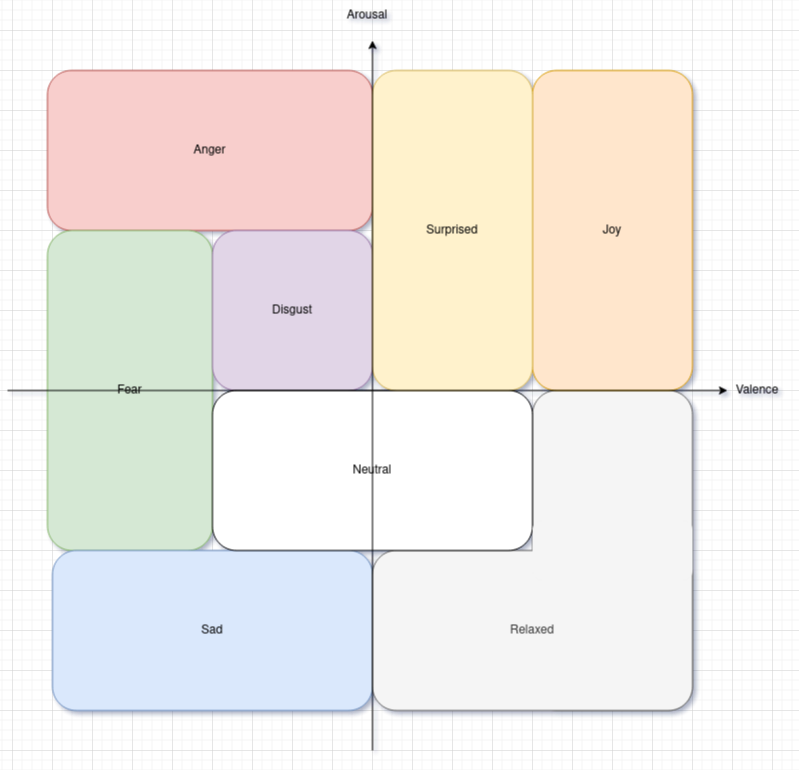
\includegraphics[width=\textwidth]{figures/va16model.png}
    \caption{Initial valence-arousal model}
    \label{fig:VAinit}
\end{figure}

\section{Eliciting Emotions}
\label{Datasets}
The value of each dataset will be weighed according to several criteria, which will be evaluated in order to ensure that the dataset is somewhat capable of evoking the desired emotions.\\\\
%Criterion regarding using video as media data
Using the first criterion, we express that a given dataset will be required to use videos as the source of media to gather emotions. This criterion was included as we wish to combine the use of picture frames and sound in order to evoke emotions. Therefore, optimal datasets would contain video media.
%Criterion towards transparency of accuracy results.
Likewise, using the second criterion, we express that the dataset will be required to display some information as to how the videos of the given dataset performed. Such a criterion will ensure transparency as to how well a given video was able to evoke the desired emotion.
%Criterion towards the length of media data for each emotion.
For the third and final criterion, a given dataset will be required to have at least 5 minutes of media data for each emotion. This criterion was included by us, as less than this amount of data will not be feasible to collect sensor data.
%How the datasets will be presented
Each dataset will be presented by a quick initial introduction to the dataset, followed by some information regarding which criteria are fulfilled in the given dataset. Lastly a paragraph about the degree of usability of the dataset. \\\\
%How we found the datasets:
The datasets were found by searching for keywords using search engines such as google scholar, where keywords were used that are related to \textit{eliciting emotion dataset}. From these initial results we also investigated references and citations. Each candidate that was found, was saved, and its associated material was investigated. 

%Criterias:
    % Atleast cover the 4 emotions regions of the valance and arousal model, i.e have atleast one emotion in each region.
    % Atlest 2-minutes of media samples for each emotions, 
%\subsection{First substantial public database}
\textit{FilmStim} is a video database containing 70 labeled clips from known movies. The dataset is made with the explicit purpose of making a freely available dataset that would be as adaptable as possible to a wide array of research questions. The labels contains six emotions: anger, fear, sadness, disgust, amusement, tenderness and additionally neutral, with clips ranging from one to seven minutes in length. The emotional responses elicited by these clips are validated by 364 participants, each viewing 10 clips. The emotional states of the participants where assessed by a emotional arousal scale, the Differential Emotions Scale and  the Positive and Negative Affect Schedule. All are self-reported by the participants. \cite{FilmStim}\newline
Although the original dataset was compiled for french language, it has since been updated with English versions where available, which is 52 out of the 70 clips. This dataset is overall very usable for this project, most of the English movie clips can be used and might even be too much for this project. \\\\
%\subsection{Music videos for emotion elicitation}
\textit{DEAP: A Database for Emotion Analysis} is a widely used multimodal dataset for the analysis of human affective state. It was originally created for the purpose of creating an adaptive music video recommendation system. For this purpose, the dataset consists of 120 one-minute excerpts from music videos, that each fit into one of 16 emotional states. Each clip is rated by 14-16 participants based on arousal, valence, and dominance. However, the range of 16 emotional states are far too specific for use in this particular study, so the dataset would need to be generalized in some way to only cover the relevant emotional states, mentioned in \cref{sec:emotionalModel}.
Furthermore, the media type of the dataset being music videos adds an additional emotional response trigger through sound elements, which is not a particularly good fit for this specific use case. The dataset is not publicly available, so it is necessary to apply to gain access, which is not guaranteed. \cite{DEAP} \newline
This dataset does not exactly fit the use case of this study, and is not publicly available. However, the described method for identifying relevant videos could be useful.  \\\\
%\subsection{Using only pictures to elicit emotions}
\textit{The IAPS: International Affective Picture System} dataset consists of pictures that are designed for studying emotions. It has been widely used in psychological research and is developed by the National Institute of Mental Health Center for Emotion and Attention at the University of Florida. The dataset consists of 956 images ranging from everyday objects to extreme and rare motives, such as mutilated bodies and erotic nudes. While previous datasets have used the valence and arousal model for assessing the emotional response of the media, the IAPS dataset uses an extended version called the VAD-model. This is a three-dimensional version of the valance and arousal model that now also includes dominance, which represents how much controlled/in-control the participant felt.\cite{IAPS}
A total of eight different emotions is covered in the dataset: amusement, anger, awe, contentment, disgust, excitement, fear, sad
This dataset fits very poorly with the use case of this study, as it only use images. Furthermore, in order to get access to the dataset, there is a 30 days processing time. \\\\
%\subsection{Real-time emotional assessment}
\textit{The CASE: Continuous affect annotations and physiological signals} for emotion analysis dataset features 30 participants who watched eight videos of 2-3 minutes, two for each of the four emotions: amusing, boring, relaxing and scary. That is one emotion for each valence/arousal quadrant. The videos were selected based on previous datasets and includes movie clips, documentaries and nature videos. To avoid the carried bias from changing videos, each participant watched the videos in random order while there was a two minute span of blue screen between each video. What is special about this dataset is that the participants log their own emotional state to a valence/arousal graph in real time using a joystick. \cite{CaseData}
This dataset is somewhat usable, while only four emotions is however in the low-end and boring and relaxing seem somewhat similar. \\\\
%\subsection{Compiling a modern database}
In \cite{FilmClips}, an attempt is made to construct a modern dataset of film clips that is able to evoke basic and complex emotions. A total of 14 emotions are measured, using the arousal and valance model. The dataset is constructed by performing two separate studies, where participants watched film clips and rated the clips according to the degree of emotion that they evoked. The paper was able to discretely elicit 11 different emotions and consists of a total of 50 film clips. Relating this to the criteria, both are fulfilled as it maps to 11 different emotions and consists of a range of videos for each emotion.\\\\
%\subsection{Eliciting emotion independent of language} 
\textit{Chen H et al.} describes the process of selecting a collection of professional and amateur videos eliciting five basic emotions: happiness, fear, disgust, anger and sadness. The dataset primarily consists of movie trailers for the professional videos and YouTube videos for the amateur videos. All videos are less than one minute.
The participants were split into three groups, with different nationalities, to ensure that the videos could elicit emotions, even though they could not understand the language. 20 professional and 20 amateur videos were chosen, and 30 participants were given the task of identifying and rating the emotions they felt. The dataset is the 40 videos with accompanying rating data. \cite{CHEN2021106662}.
This dataset is somewhat usable in that it aims to elicit five strong and different emotions. Unfortunately some videos are very short, down to 5 seconds. However, there are many videos for each emotion, allowing us to choose the ones that makes most sense or maybe put some of the short videos together in sequence. \\\\

\subsection{Our selection}
Based on the datasets we have just presented we will now explain how we construct the dataset that we will use for our experiments. None of the above datasets cover all the emotional states we want to cover. Because of this we will use the videos from those datasets, when publicly available, that relate to the emotions we aim for. Some emotions have many related videos. For these we will choose two videos for each emotion, choosing those best shown to elicit the relevant emotion. \Cref{tab:videos} show which videos for each dataset are relevant for the chosen emotions and which we choose for our dataset.

\begin{table}[]
    \centering
    \begin{tabular}{|c|c|c|c|c|}
        \hline
        %Happy
         Origin & Emotion & Length & Evaluation & Chosen  \\ \hline
         Les trois frères & Happy & 2:24 & 4.55    & No \\ \hline
         The Dinner Game & Happy & 1:40 & 4.5    & No \\ \hline
         La cité de la peur & Happy & 2:13 & 4.29   & No \\ \hline
         The Visitors & Happy & 2:09 & 4.27   & No \\ \hline
         A Fish Called Wanda & Happy & 2:53 & 3.81   & No \\ \hline
         Benny and Joon & Happy & 2:01 & 3.73   & No \\ \hline
         Something About Mary[2] & Happy & 2:26 & 3.68   & No \\ \hline
         Something About Mary[1] & Happy & 2:55 & 3.61   & No \\ \hline
         When Harry Met Sally & Happy & 2:45 & 3.55   & No \\ \hline
         Le Pari & Happy & 1:47 & 3.48   & No \\ \hline
         %Anger
         Schindler’s List [2] & Anger & 1:55 & 2.19   & No \\ \hline
         Sleepers & Anger & 2:20 & 2.72   & Yes \\ \hline
         Leaving Las Vegas & Anger & 2:30 & 2.00   & No \\ \hline
         American History X & Anger & 1:17 & 1.94   & Yes \\ \hline
         Schindler’s List [1] & Anger & 1:18 & 1.70   & No \\ \hline
        Schindler’s List [3] & Anger & 1:30 & 1.33   & No \\ \hline
         Man Bites Dog [1] & Anger & 1:54 & 1.30   & No \\ \hline
         In the Name of the Father & Anger & 3:30 & 1.10   & No \\ \hline
         Seven [1] & Anger & 1:53 & 0.99   & No \\ \hline
         A Perfect World & Anger & 4:27 & 0.69   & No \\ \hline
         %Sadness
         City of Angels & Sadness & 4:15 & 2.32   & No \\ \hline
         Dangerous Mind & Sadness & 2:08 & 2.29   & No \\ \hline
         Philadelphia & Sadness & 5:28 & 2.27   & No \\ \hline
         The Dead Poets Society [1] & Sadness & 4:14 & 1.64   & No \\ \hline
         The Dreamlife of Angel & Sadness & 2:41 & 1.46   & No \\ \hline
         Dead Man Walking & Sadness & 6:40 & 1.02   & No \\ \hline
         The Professional [1] & Sadness & 2:44 & 0.93   & No \\ \hline
         Schindler’s List [1] & Sadness & 1:18 & 0.88   & No \\ \hline
         A Perfect World & Sadness & 4:27 & 0.84   & No \\ \hline
         Life is Beautiful [1] & Sadness & 2:07 & 0.81   & No \\ \hline
         %Fear
          The Blair Witch Project & Fear & 3:57 & 2.93   & No \\ \hline
          The Shining & Fear & 4:27 & 2.77   & No \\ \hline
          Scream 1 & Fear & 6:33 & 2.38   & No \\ \hline
          Misery & Fear & 3:31 & 2.32   & No \\ \hline
          Scream 2 & Fear & 3:35 & 2.12   & No \\ \hline
          Child’s Play 2: Chucky’s Back & Fear & 1:05 & 2.02   & No \\ \hline
          Copycat & Fear & 2:23 & 1.96   & No \\ \hline
          The Dentist & Fear & 0:56 & 1.91   & No \\ \hline
          The Exorcist & Fear & 1:41 & 1.83   & Yes \\ \hline
          Seven [2] & Fear & 1:43 & 1.81   & No \\ \hline
          %Disgust
          Trainspotting [2] & Disgust & 1:44 & 4.07   & Yes \\ \hline
          Seven [3] & Disgust & 3:19 & 3.41   & No \\ \hline
          Hellraiser & Disgust & 1:30 & 3.14   & No \\ \hline
          Man Bites Dog [1] & Disgust & 1:54 & 2.99   & No \\ \hline
          Seven [2] & Disgust & 1:43 & 2.90   & No \\ \hline
          The Dentist & Disgust & 0:56 & 2.84   & No \\ \hline
          American History X & Disgust & 1:17 & 2.77   & No \\ \hline
          Sleepers & Disgust & 2:20 & 2.76   & No \\ \hline
          Misery & Disgust & 3:31 & 2.69   & No \\ \hline
          The Silence of the Lambs & Disgust & 4:27 & 2.54   & No \\ \hline
          The Silence of the Lambs & Disgust & 4:27 & 2.54   & No \\ \hline
          
          
    \end{tabular}
    \caption{Relevant videos from the FilmStim dataset. Evaluation is a 1-7 scale \cite{FilmStim}}
    \label{tab:videos}
\end{table}


\begin{table}[]
    \centering
    \begin{tabular}{|c|c|c|c|c|}
        %Happy
        \hline
         Origin & Emotion & Length & Evaluation & Chosen  \\ \hline
         %FilmClips
          Enough & Anger & 1:43 & 8.0  & No \\ \hline
          American History X & Disgust & 1:23 & 8.3  & No \\ \hline
          Cairo Time X & Disgust & 0:54 & 7.1  & No \\ \hline
          Limitless (blood) & Disgust & 0:58 & 7.7  & No \\ \hline
          Slumdog Millionaire (blinded) & Disgust & 0:56 & 8.3  & Yes\\ \hline
          50 First Dates & Joy & 0.42 & 7.2  & No \\ \hline
          Coach Carter (honoring coach) & Joy & 0:43 & 6.4  & Yes \\ \hline
          Coach Carter (winning basket) & Joy & 1:33 & 7.3  & Yes \\ \hline
          Forrest Gump (reunion) & Joy & 0:48 & 7.5  & Yes \\ \hline
          Lottery Ticket & Joy & 1:13 & 7.5  & No \\ \hline
          My Sister's keeper (trampoline) & Joy & 0:26 & 6.9  & No \\ \hline
          Short Term 12 & Joy & 0:52 & 6.6  & No \\ \hline
          Soul Surfer (homeless girl) & Joy & 1:45 & 7.6  & Yes \\ \hline
          Soul Surfer (surfing) & Joy & 1:47 & 7.4  & No \\ \hline
          Wedding Crashers & Joy & 1:02 & 6.7  & No \\ \hline
          A Good Year & Neutral & 1:32 & 4.8  & No \\ \hline
          Ex Machina & Neutral & 0.45 & 6.9  & Yes \\ \hline
          Labor Day & Neutral & 0:32 & 5.7  & No \\ \hline
          Rudderless (buisness meeting) & Neutral & 0:29 & 6.8  & Yes \\ \hline
          The Other Woman & Neutral & 0.45 & 5.4  & No \\ \hline
          Blood Diamond (begging) & Sad & 0:55 & 6.5  & No \\ \hline
          Detachment & Sad & 1:33 & 7.2  & No \\ \hline
          My Sister's Keeper (cancer impact) & Sad & 2:00 & 7.7  & No \\ \hline
          The Mist (family) & Sad & 2:41 & 7.0  & No \\ \hline
          %Fear
          Insidious & Fear & 1:46 & 6.95  & Yes \\ \hline
          No Escape & Fear & 0:29 & 6.02  & No \\ \hline
          The Conjuring & Fear & 2:06 & 7.3  & Yes \\ \hline
          The Life Before Her eyes & Fear & 5:08 & 7.2  & No \\ \hline
          %Sad
          Freedom Writers (diary) & Sad & 2:00 & 6.51  & No \\ \hline
          I Am Sam & Sad & 1:12 & 7.9  & Yes \\ \hline
          My Sister's Keeper (doctor)  & Sad & 1:09 & 7.9  & No \\ \hline
          Still Alice & Sad & 1:26 & 7.5  & No \\ \hline
          The Pursuit of Happyness (subway) & Sad & 2:39 & 7.6  & Yes \\ \hline
          Deep Blue Sea & Surprise & 1:57 & 7.7  & Yes \\ \hline
          Joe & Surprise & 0:22 & 7.4  & No \\ \hline
          Meet Joe Black & Surprise & 2:27 & 6.9  & No \\ \hline
          One day & Surprise & 0:25 & 7.5  & Yes \\ \hline
          The Call (parking garage) & Surprise & 0:24 & 6.4  & No \\ \hline
    \end{tabular}
    \caption{Relevant videos from the FilmClips dataset. Evaluation is a 1-9 scale \cite{FilmClips}}
    \label{tab:my_label}
\end{table}


\begin{table}[]
    \centering
    \begin{tabular}{|c|c|c|c|c|}
        %Happy
        \hline
        Origin & Emotion & Length & Evaluation  & Chosen  \\ \hline
        Forrest Gump & Joy & 0:32 & 3.5 & No \\ \hline
        Playing with Fire & Joy & 0:21 & 4 & No \\ \hline
        Slumdog Millionaire & Joy & 0:25 & 4 & No \\ \hline
        Home Alone 2: Lost in New York & Joy & 0:42 & 3.5 & No \\ \hline
        Countdown & Fear & 0:29 & 4 & No \\ \hline
        Doctor Sleep & Fear & 0:15 & 4 & No \\ \hline
        It & Fear & 0:21 & 4 & No \\ \hline
        Scary Stories to Tell in the Dark & Fear & 0:18 & 4 & No \\ \hline
        Jennifer's Body & Disgust & 0:05 & 3 & No \\ \hline
        Midsommar & Disgust & 0:05 & 4 & No \\ \hline
        The Shining & Disgust & 0:12 & 3 & No \\ \hline
        The Babysitter & Disgust & 0:10 & 3 & No \\ \hline
        Argo & Anger & 0:19 & 3 & No \\ \hline
        Chicago & Anger & 0:05 & 3.5 & No \\ \hline
        12 Years a Slave & Anger & 0:41 & 4 & No \\ \hline
        The King's Speech & Anger & 0:21 & 3.5 & No \\ \hline
        Titanic & Sadness & 0:30 & 3.5 & No \\ \hline
        Moonlight & Sadness & 0:42 & 4 & No \\ \hline
        Crash & Sadness & 0:41 & 4 & No \\ \hline
        Unforgiven & Sadness & 0:37 & 3 & No \\ \hline
    \end{tabular}
    \caption{Relevant videos from the Chen et al. dataset. Evaluation is a 1-5 scale \cite{CHEN2021106662}}
    \label{tab:my_label}
\end{table}

\begin{table}[]
    \centering
    \begin{tabular}{|c|c|c|c|c|c|c|}
        %Happy
        \hline
        ID & Origin & Emotion & Length & Evaluation & Source\\ \hline
        1 & The Pursuit of Happyness (subway) & Sad & 4:20 & 7.6  & FilmClips \cite{FilmClips} \\ \hline
        2 & I Am Sam & Sad & 2:16 & 7.9  & FilmClips \cite{FilmClips}\\ \hline
        3 & The Conjuring & Fear & 3:04 & 7.3  & FilmClips \cite{FilmClips}  \\ \hline
        4 & Insidious & Fear & 3:08 & 6.95  & FilmClips \cite{FilmClips} \\ \hline
        5 & Ex Machina & Neutral & 0:59 & 6.9  & FilmClips \cite{FilmClips} \\ \hline
        6 & Rudderless (buisness meeting) & Neutral & 0:43 & 6.8  & FilmClips \cite{FilmClips} \\ \hline
        7 & Soul Surfer (homeless girl) & Joy & 2:31 & 7.6  & FilmClips \cite{FilmClips} \\ \hline
          %Coach Carter (honoring coach) & Joy & 0:43 & 6.4  & FilmClips \cite{FilmClips} & Yes \\ \hline
          %Coach Carter (winning basket) & Joy & 1:33 & 7.3  & FilmClips \cite{FilmClips} & Yes \\ \hline
        8 & Forrest Gump (reunion) & Joy & 1:12 & 7.5  & FilmClips \cite{FilmClips} \\ \hline
        9 & Slumdog Millionaire (blinded) & Disgust & 1:46 & 8.3  & FilmClips \cite{FilmClips} \\ \hline
        10 &  Trainspotting [2] & Disgust & 1:14 & 4.07  & FilmStim \cite{FilmStim} \\ \hline
        11 & Sleepers & Anger & 2:34 & 2.72  & FilmStim \cite{FilmStim}  \\ \hline
        12 & American History X & Anger & 1:31 & 1.94  & FilmStim \cite{FilmStim} \\ \hline
        13 & One day & Surprise & 0:37 & 7.5 & FilmClips \cite{FilmClips}\\ \hline
        14 & Deep Blue Sea & Surprise & 2:14 & 7.7 & FilmClips \cite{FilmClips} \\ \hline
        15 & Relaxing Piano Music - Nature Scenes & Relaxed & 2:10 & N/A & CASE \cite{CaseData}  \\ \hline
        16 & Relaxing Sunset To Nightfall Relaxation Meditation & Relaxed & 2:10 & N/A & CASE \cite{CaseData} \\ \hline
    \end{tabular}
    \caption{Chosen videos}
    \label{tab:my_label}
\end{table}

Total time is 32 minutes and 29 seconds

%\subsection{CLAS (2019)}
%The CLAS dataset is a multimodal resource, which was developed for research in automated recognition of some specific states of mind. The dataset consists of recordings of Electrocardiography (ECG), Plethysmography (PPG), ElectroDermal Activity (EDA), as well as accelerometer data. A total of 62 volunteers were recorded while doing 3 interactive tasks, and two perceptive tasks. The interactive task aims to trigger some cognitive effort, which in this case is triggered by solving math problems, logic problems, and a stroop test. The perceptive task makes use of image- and audio-stimuli in order to evoke emotions which are measured using the valance- and arousal model. Combining these two kinds of tasks enables for a multifaceted evaluation of specific states of mind. The dataset measures xx emotions by... , and therefore fulfills the first criterion. The second criterion, however, is not fulfilled as the participants was asked to do tasks, instead of exposed to media data. As a result of this, the dataset was discarded.
%This dataset has some very intriguing aspects, both in terms of how the dataset has been collected, but also the metrics by which the results are measured. However, the data which has been gathered in the dataset consists of only ECG, PPG, EDA and accelerometer. Since this paper has committed to using PPG and GSR data, it is not an optimal solution. 
%Another solution could be to use the data that has been used for collecting and use this data to conduct a study where GSR and PPG is collected. This would save time, as a big part of the data collection would be completed. This solution is not feasible as well, as this data is not available.
%\cite{CLAS}